\documentclass[12pt]{article}

\usepackage{sbc-template}

\usepackage{graphicx,url}

\usepackage[brazil]{babel}   
%\usepackage[latin1]{inputenc}  
\usepackage[utf8]{inputenc}  
% UTF-8 encoding is recommended by ShareLaTex

\usepackage{amssymb}
     
\sloppy

\title{Trabalho Prático 1 - Programação Genética para Regressão Simbólica}

\author{Hugo Araujo de Sousa}

\address{
  Computação Natural (2017/2) \\
  Departamento de Ciência da Computação \\
  Universidade Federal de Minas Gerais (UFMG)
  \email{hugosousa@dcc.ufmg.br}
}

\begin{document} 

\maketitle
     
\begin{resumo} 
  Este trabalho objetiva o desenvolvimento de conceitos fundamentais na
  aplicação de Programação Genética para resolução do problema de Regressão
  Simbólica. A estrutura geral do algoritmo de Programação Genética é
  apresentada, a mesma é modelada para o problema de Regressão Simbólica
  e, finalmente, utilizando-se de dados de teste, são realizados experimentos e
  análise de resultados.
\end{resumo}

\section{INTRODUÇÃO}

Como definido por \cite{plmgp:08}, Programação Genética é um conjunto de técnicas
de Computação Evolucionária que permite resolver problemas de forma automática.
Dessa forma, o usuário não precisa, de antemão, determinar a forma ou estrutura 
que a solução para um determinado problema terá.

Em Programação Genética, cada possível solução para um problema é definida como um
indivíduo. Inicialmente, é criado um grupo aleatório desses indivíduos, chamado de
população. Cada um desses indivíduos é avaliado para determinar o quão próximos da
solução ótima do problema eles estão. Baseado nessa proximidade, esses indivíduos
são "evoluídos", criando assim novas gerações de indivíduos que passam pelo mesmo
processo por um número determinado de vezes. Finalmente, o melhor indivíduo obtido
ao final dessas gerações é retornado ao usuário como a solução do problema em questão.

Um dos problemas que podemos resolver com Programação Genética é o de Regressão Simbólica.
Nele, o usuário possui um conjunto de m amostras provenientes de uma função desconhecida
que recebe n valores reais e retorna um único valor real. O objetivo então é encontrar a
expressão simbólica dessa função que melhor se ajusta às amostras fornecidas.

\section{MODELAGEM} \label{sec:model}

\subsection{Indivíduos} \label{sec:ind}

A primeira decisão de implementação em Programação Genética é a de como representar
os indivíduos que representarão soluções para o problema a ser resolvido. Para o
problema de Regressão Simbólica, uma solução é uma função do tipo
$ f:\mathbb{R}^{m} \rightarrow \mathbb{R} $. Dessa forma, a representação escolhida
para representar uma função que resolva o problema é a de uma árvore onde os nós
internos representam operadores e os nós folha são formados por terminais, isto é,
variáveis da função ou constantes. Para os nós que representam operadores, os nós filhos
serão os operandos. A Figura \ref{fig:gp_ind} mostra um exemplo de indivíduo com essa
configuração.

\begin{figure}[ht]
\centering
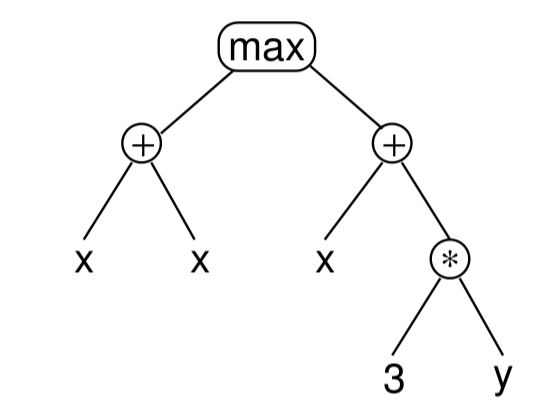
\includegraphics[width=.7\textwidth]{gp_ind.png}
\caption{Exemplo de um indivíduo em Programação Genética que representa a expressão
simbólica $\mathbf{max(x+x, x+3*y)}$.}
\label{fig:gp_ind}
\end{figure}

Para este trabalho, o conjunto de terminais e operadores escolhidos é mostrado a seguir:

\begin{itemize}
 \item \textbf{Operadores:}
 \begin{itemize}
  \item \textbf{Binários:}
   \begin{itemize}
    \item \textbf{+}: Operador de adição.
    \item \textbf{-}: Operador de subtração.
    \item \textbf{*}: Operador de multiplicação.
    \item \textbf{/}: Operador de divisão.
    \item \textbf{\^}: Operador de exponenciação.
   \end{itemize}
   
   \item \textbf{Unários:}
   \begin{itemize}
    \item \textbf{log}: Função logaritmo (base e).
    \item \textbf{sin}: Função seno.
    \item \textbf{cos}: Função cosseno.
    \item \textbf{sqrt}: Função raiz quadrada.
   \end{itemize}

 \end{itemize}
 
 \item \textbf{Terminais:}
 \begin{itemize}
  \item \textbf{Constantes}: Valores reais aleatoriamente gerados.
  \item \textbf{Variáveis}: Representam variáveis da função a ser aproximada.
  O número de variáveis aleatoriamente geradas é igual ao número de variáveis
  de entrada da função que o usuário deseja aproximar.
 \end{itemize}
 
\end{itemize}

\subsection{Fitness}

Como dito anteriormente, cada indivíduo presente em uma determinada geração
deverá ser avaliado para obter uma medida de quão bem esse indivíduo aproxima
a função cujos valores de entrada e saída são fornecidos pelo usuário. O critério
de avaliação da qualidade do indivíduo, também conhecido como fitness, para este
trabalho, será dado pela raiz quadrada do erro quadrático médio (RMSE).

\begin{center}
 \begin{math}
  f(Ind) = \sqrt{\frac{1}{N}\sum_{n=1}^{N}(Eval(Ind, x) - y)^2}
  \end{math}
\end{center}

onde Ind é o indivíduo sendo avaliado, $ Eval(Ind, x) $ avalia o indivíduo Ind
no conjunto de entrada fornecido $ x $, $ y $ é a saída correta da função para 
a entrada $ x $ e $ N $ é o número de exemplos fornecidos.

Dessa forma, a função $ Eval(Ind, x) $ vai atribuir os valores em $ x $ às
variáveis presentes em Ind, e retornar o valor $ y $ correspondente à saida
da expressão simbólica que Ind representa para $ x $.

\subsection{Geração de População Inicial}

Existem vários métodos para geração da população inicial de indivíduos que serão
evoluídos ao longo das gerações em que o programa executará. Neste trabalho é usada
uma combinação de dois deles:

\begin{itemize}
 \item \textbf{Full:} Gera indivíduos cuja expressão simbólica é dada por uma árvore
 completa, i.e., todas as folhas estão na mesma profundidade.
 \item \textbf{Grow:} Gera indivíduos com formas e tamanhos variados, uma vez que
 os nós são selecionados tanto dos operadores quanto dos terminais até que a profundidade
 limite é atingida. Quando isso acontece, somente terminais são selecionados para compor
 nós.
\end{itemize}

Para garantir uma diversidade elevada de indivíduos na população inicial, é usado o
método \textbf{Ramped Half-and-Half}, que combina os métodos Full e Grow, gerando
metade da população com o primeiro e metade com o segundo.

\subsection{Evolução}

Uma vez gerada a população de indivíduos, o algoritmo de Programação Genética entra
em um laço de repetição, evoluindo indivíduos e gerando populações cada vez melhores.
A evolução dos indivíduos presentes em uma população se dá através de seleção e aplicação
de operadores genéticos.

\subsubsection{Seleção}

É desejável que, a cada geração, sejam mantidas as características dos indivíduos que
apresentam melhor fitness (menor, no caso da regressão simbólica). Logo, é necessário
incluir um mecanismo que permita selecionar, dada uma certa população, indivíduos que
se destacam.

Nesse trabalho, o mecanismo de seleção implementado foi o de \textbf{Seleção por Torneio}.
Esse tipo de seleção escolhe um grupo aleatório de tamanho $ k $ dentre os indivíduos
de uma população e retorna aquele, dentre os $ k $ escolhidos, que tenha a melhor fitness.

Além disso, foi adicionado ao projeto a possibilidade de se utilizar o conceito de 
\textbf{elitismo}. Com esse conceito, os $ n $ melhores indivíduos de cada geração são
simplesmente passados para a geração seguinte, onde $ n $ é um parâmetro definido pelo
usuário.

\subsubsection{Operadores Genéticos}

A partir dos indivíduos selecionados em cada geração, aplica-se um conjunto de operadores
genéticos sobre os mesmos, a fim de garantir que novos indivíduos (baseados nesses que
se destacaram em cada geração) possam surgir. Cada um desses operadores genéticos contribui
de uma forma para o algoritmo e é aplicado seguindo uma certa probabilidade pré-definida.

Os operadores genéticos implementados nesse trabalho são apresentados a seguir.

\begin{itemize}
 \item \textbf{Cruzamento:} Dois indivíduos são selecionados e partes desses indivíduos
 (subárvores) são trocadas de lugar, gerando dois novos indivíduos. Os indivíduos pais
 não são alterados nesse processo.
 
 \item \textbf{Mutação:} Uma parte aleatória de um indivíduo selecionado é alterada.
 Essa parte pode ser removida, expandida, simplesmente ter seu conteúdo trocado, etc.
 Para o trabaho, foi implementada mutação de subárvore, onde um nó é escolhido para
 ser expandido, sendo criada uma nova subárvore a partir do mesmo.
 
 \item \textbf{Reprodução:} Um indivíduo selecionado é simplesmente passado adiante para
 a próxima geração.
\end{itemize}


\section{IMPLEMENTAÇÃO}

\begin{figure}[ht]
\centering
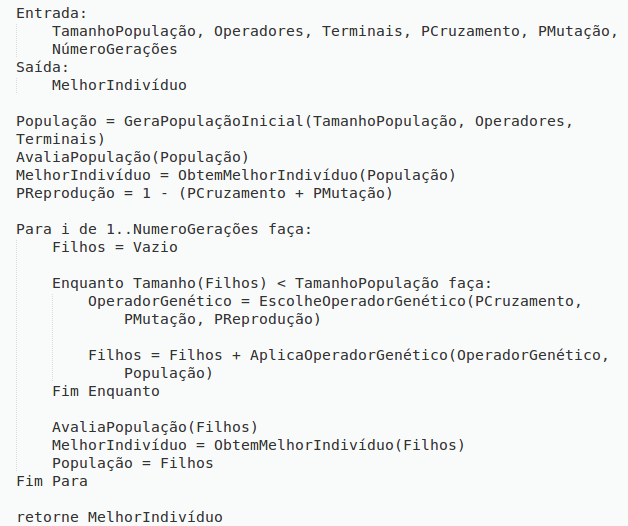
\includegraphics[width=1\textwidth]{gp_code.png}
\caption{Pseudocódigo para um algoritmo de Programação Genética.}
\label{fig:gp_code}
\end{figure}

Dada a modelagem do problema mostrada na Seção \ref{sec:model} o algoritmo principal
segue o pseudocódigo mostrado na Figura \ref{fig:gp_code}.

Para o trabalho, o algoritmo então foi implementado usando a linguagem Python 3.

A classe \textbf{Individual} representa um indivíduo conforme descrito na Seção
\ref{sec:ind}, e é a principal do projeto. Nela estão presentes todos os métodos 
para construção de indivíduos, populações, avaliação de indivíduos, etc.

Algumas decisões de implementação importantes são discutidas a seguir:

\begin{itemize}
 \item Biblioteca Numpy utilizada no projeto intensivamente. É com ela que toda a geração
 de números aleatórios é feita e as operações dos nós são feitas.
 
 \item As constantes geradas para nós terminais são números reais no intervalo
 $ [-10, 10] $.
 
 \item A fim de otimizar a cópia dos indivíduos pais durante a etapa de cruzamento,
 foi criada uma função copy, mais específica do que a alternativa deepcopy da linguagem.
 
 \item No método de criação de indivíduos Grow, os tipos dos nós são gerados aleatoriamente
 com probabilidades $ 0.8, 0.1 $ e $ 0.1 $ para nós de operadores, variáveis e constantes,
 respectivamente.
 
 \item Para evitar que os indivíduos gerados cresçam indefinidamente, existe uma penalidade
 para indivíduos que excedam um tamanho limite. Esse tamanho (número de nós) máximo é dado
 por $ 2^(D) - 1 $, onde $ D $ é a profundidade máxima das árvores geradas. Indivíduos que
 ultrapassem esse tamanho recebem fitness infinita.
 
 \item A produndidade máxima dos indivíduos não é variada, tendo valor $ 7 $.
\end{itemize}


\section{ESTRUTURA DO PROJETO E EXECUÇÃO}

Os arquivos de código-fonte do projeto se encontram na pasta \textbf{src}. Nela, o
código-fonte é dividido da seguinte forma:

\begin{itemize}
 \item \textbf{individual.py:} Define a classe Individual e todos os métodos necessários
 para criação e avaliação de indivíduos e criação de populações.
 
 \item \textbf{gp.py:} Métodos auxiliares para Programação Genética, tais como seleção
 por torneio, avaliação de população e operadores genéticos.
 
 \item \textbf{tp1.py:} Programa principal. Nele está implementado o algoritmo principal
 de Programação Genética, além de todos os métodos de manipulação de entrada e saída.
\end{itemize}

\subsection{Execução e Parâmetros}

A fim de facilitar a execução do programa, foram definidos parâmetros para alterar 
alguns pontos chave para Programação Dinâmica. São eles:

\begin{itemize}
 \item \textbf{Semente:} Número inteiro usado na geração de números aleatórios durante a 
 execução do programa. Note que, mantendo todos os outros parâmetros fixos, a saída
 do programa para uma mesma entrada e valor de seed será sempre igual. A semente
 da execução pode ser definida com a flag \textbf{-s} e tem valor padrão $ 0 $.
 
 \item \textbf{Tamanho da população:} Número inteiro que determina o tamanho de indivíduos
 presente em cada geração. Pode ser definido com a flag \textbf{-p} e tem valor padrão
 $ 54 $.
 
 \item \textbf{Tamanho do torneio:} Número de indivíduos que competem em cada seleção
 por torneio. Definido com a flag \textbf{-k} e tem valor padrão $ 7 $.
 
 \item \textbf{Número de gerações:} Define o número de gerações pelo qual o programa
 deve executar. Definido com a flag \textbf{-g} e tem valor padrão $ 10 $.
 
 \item \textbf{Taxa de cruzamento:} Probabilidade de usar o operador de cruzamento para
 gerar filhos em cada geração. Definida com a flag \textbf{-c}, valor padrão $ 0.9 $.
 
 \item \textbf{Taxa de mutação:} Probabilidade de usar o operador de mutação para
 gerar filhos em cada geração. Definida com a flag \textbf{-m}, valor padrão $ 0.05 $.
 
 \item \textbf{Tamanho da elite:} Tamanho da elite a ser transferida automaticamente para
 a próxima geração, a cada geração. Definido com a flag \textbf{-e}, valor padrão $ 2 $.
 Note que para desativar o elitismo, basta usar \textbf{-e 0}.
 
\end{itemize}

Note que a taxa de reprodução não é definida pelo usuário, mas calculada em função das 
taxas de cruzamento e mutação, como mostrado na Figura \ref{fig:gp_code}.

Para executar o programa, o comando abaixo é usado:

\begin{center}
 tp1.py [\-h] [\-s RSEED] [\-p POP\_SIZE] [\-k KTOUR] [\-g NGEN] [\-c CROSSR]
              [\-m MUTR] [\-e ELIT]
              train\_file test\_file
\end{center}

Onde RSEED indica a semente, POP\_SIZE o tamanho da população, KTOUR o número de competidores
em torneios, NGEN o número de gerações, CROSSR a probabilidade de cruzamento, MUTR a probabilidade
de mutação, ELIT o tamanho da elite em cada geração, train\_file o nome do arquivo com as
entradas de treino e test\_file o nome do arquivo com as entradas de teste.

Todos os parâmetros entre colchetes acima são opcionais.

\subsection{Entrada e Saída}

Os arquivos de entrada, tanto de treino quanto de teste, devem possuir a mesma estrutura.
O arquivo de treino é usado para evoluir as soluções do programa até o número máximo de
gerações ser alcançado. Quando essa etapa é finalizada, as melhores soluções encontradas
são avaliadas com o arquivo de teste.

Em ambos os arquivos, cada linha representa uma amostra da função a se aproximar. Sendo
$ x + 1 $ valores de ponto flutuante separados por vírgula, onde $ x $ é o número de variáveis
da função. A última coluna, então, representa a saída $ y $ da função para os valores de entrada
das colunas anteriores.

Em relação à saída do programa, é impresso, a cada geração, um resumo de estatísticas.
Primeiramente é impresso o número da geração atual, em seguida o valor da fitness do melhor
indivíduo da geração, da fitness do pior indivíduo, a fitness média considerando todos
os indivíduos da geração, o número de indivíduos repetidos, a taxa de melhoria para mutação
e cruzamento.

As taxas de melhoria são calculadas da seguinte forma:

\begin{center}
 \begin{math}
  Imp(op) = \frac{NImp}{NGen}
 \end{math}
\end{center}

Sendo Imp(op) a taxa de melhoria para o operador op, NGen representa o número de indivíduos
criados em determinada geração utilizando-se o operador genético op e NImp o número, dentre
esses indivíduos gerados, daqueles que apresentaram fitness melhor do que seus pais (indivíduos
sobre os quais o operador op foi aplicado).

Exemplo de estatísticas para uma certa geração:

\begin{center}
  Generation 7\\
  Best fitness: 2.77477679664e-09\\
  Worst fitness: inf\\
  Average fitness: 1.70803185868e+17\\
  Number of repeated individuals: 15\\
  Mutation improvement rate: 0.0\% \\
  Crossover improvement rate: 6.25\%
\end{center}

\section{EXPERIMENTOS}

Nessa seção serão apresentados os experimentos realizados. Todos eles foram executados em
uma máquina Intel Core i7-5500U, 2.40GHz, 4 cores, 8GB de memória RAM e sistema operacional
ubuntu 14.04 LTS.

\subsection{Metodologia}

Muitas instâncias de teste foram executadas para cada uma das bases de teste. Alguns exemplos
de saídas obtidas estão presentes na pasta \textbf{test}.

Um script para teste de todas as bases presentes no diretório \textbf{datasets} com todas as
possíveis configurações de parâmetro e 30 execuções/sementes foi desenvolvido. Para executá-lo,
basta digitar o comando a seguir no terminal:

\begin{center}
 ./run\_tests.py
\end{center}

A metodologia para execução dos testes seguiu muitas das orientações presentes em \cite{clalg:11}.

\subsection{Experimentos}

Abaixo são mostrados os principais experimentos realizados. Os resultados são apresentados
na Seção \ref{sec:result}. Os valores apresentados foram obtidos da média de 30 execuções.

\begin{itemize}
 \item \textbf{Experimento 1:} No primeiro experimento, objetivou-se simplesmente a verificação
 de convergência da melhor indivíduo em relação ao número de gerações.Os parâmetros utilizados
 estão listados abaixo. \\
 
 \begin{itemize}
  \item Base keijzer-7:
  
  Tamanho da população: \\
  Competidores em torneios: \\
  Número de gerações: \\
  Taxa de cruzamento: \\
  Taxa de mutação: \\
  Tamanho da elite: \\
 
  \item Base keijzer-10:
  
  Tamanho da população: 100\\
  Competidores em torneios: 2\\
  Número de gerações: 100\\
  Taxa de cruzamento: 0.8\\
  Taxa de mutação: 0.1\\
  Tamanho da elite: 2\\
  
  \item Base house:
  
  Tamanho da população: 100\\
  Competidores em torneios: 7\\
  Número de gerações: 50\\
  Taxa de cruzamento: 0.9\\
  Taxa de mutação: 0.05\\
  Tamanho da elite: 2\\
  
 \end{itemize}
 
 \item \textbf{Experimento 2:} Com o experimento 2, procurava-se determinar a melhor configuração,
 dos parâmetros de número de gerações e tamanho de população inicial. Para isso, a base house foi
 utilizada. Os parâmetros são mostrados abaixo.
 
 Tamanho da População: \{5, 100, 500\} \\
 Competidores em torneios: 7 \\
 Número de gerações: 50 \\
 Taxa de cruzamento: 0.8 \\
 Taxa de mutação: 0.1 \\
 Tamanho da elite: 2 \\
 
 \item \textbf{Experimento 3:} Já com valores de tamanho de população e número de gerações fixados,
 o próximo passo foi determinar os parâmetros de probabilidade de aplicação dos operadores genéticos.
 
 Foram testadas duas configurações:
 
 Tamanho da População: 50 \\
 Competidores em torneios: 7 \\
 Número de gerações: 50 \\
 Cruzamento, mutação: \{0.9, 0.05\} e \{0.6, 0.3\} \\
 Tamanho da elite: 2 \\
 
 \item \textbf{Experimento 4:} Uma vez estabelecidas as taxas de cruzamento e mutação que promovem
 um melhor resultado do programa, é necessário testar os valores de tamanho de torneio. Esse valor
 refere-se ao número de competidores que competem a cada seleção de indivíduos por torneio.
 
 \item \textbf{Experimento 5:} Em seguida, vemos como é o comportamento do melhor indivíduo de
 cada geração, e, consequentemente, da melhor fitness, utilizando ou não de elitismo.
 
 \item \textbf{Experimento 6:} Uma vez que a diversidade dos indivíduos presentes em uma população
 cai muito, a melhor fitness de cada geração tende a permanecer sem grandes modificações. Para este
 trabalho, a única medida, ainda que não muito eficaz, de diversidade, é o número de indivíduos
 repetidos. Um indivíduo é considerado repetido aqui quando já existe na mesma geração um indivíduo
 que apresenta a mesma estrutura (mesma expressão simbólica - genótipo do indivíduo).
 
\end{itemize}


\section{RESULTADOS} \label{sec:result}

\subsection{Experimento 1: Convergência de melhor fitness}

Esse experimento comprova que, de fato, o algoritmo implementado leva as populações
geradas inicialmente a convergirem eventualmente, tentando sempre se aproximar do valor
ótimo de fitness igual a zero para as bases keijzer (o que indica que a solução ótima
pode ter sido encontrada).

\begin{figure}[ht]
  \centering
  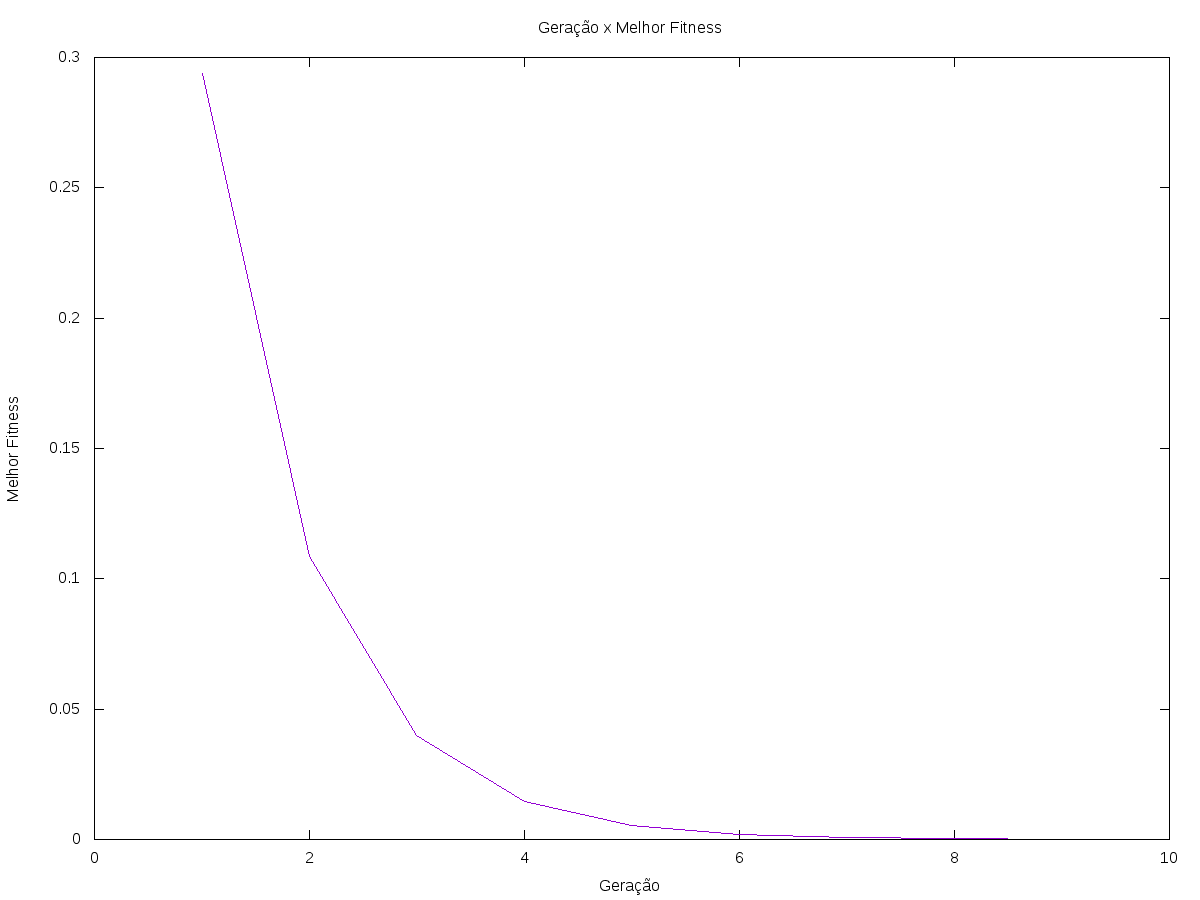
\includegraphics[width=1\textwidth]{exp1k7.png}
  \caption{Experimento 1: Geração x Melhor Fitness para base keijzer-7.}
  \label{fig:exp1k7}
\end{figure}

\begin{figure}[ht]
  \centering
  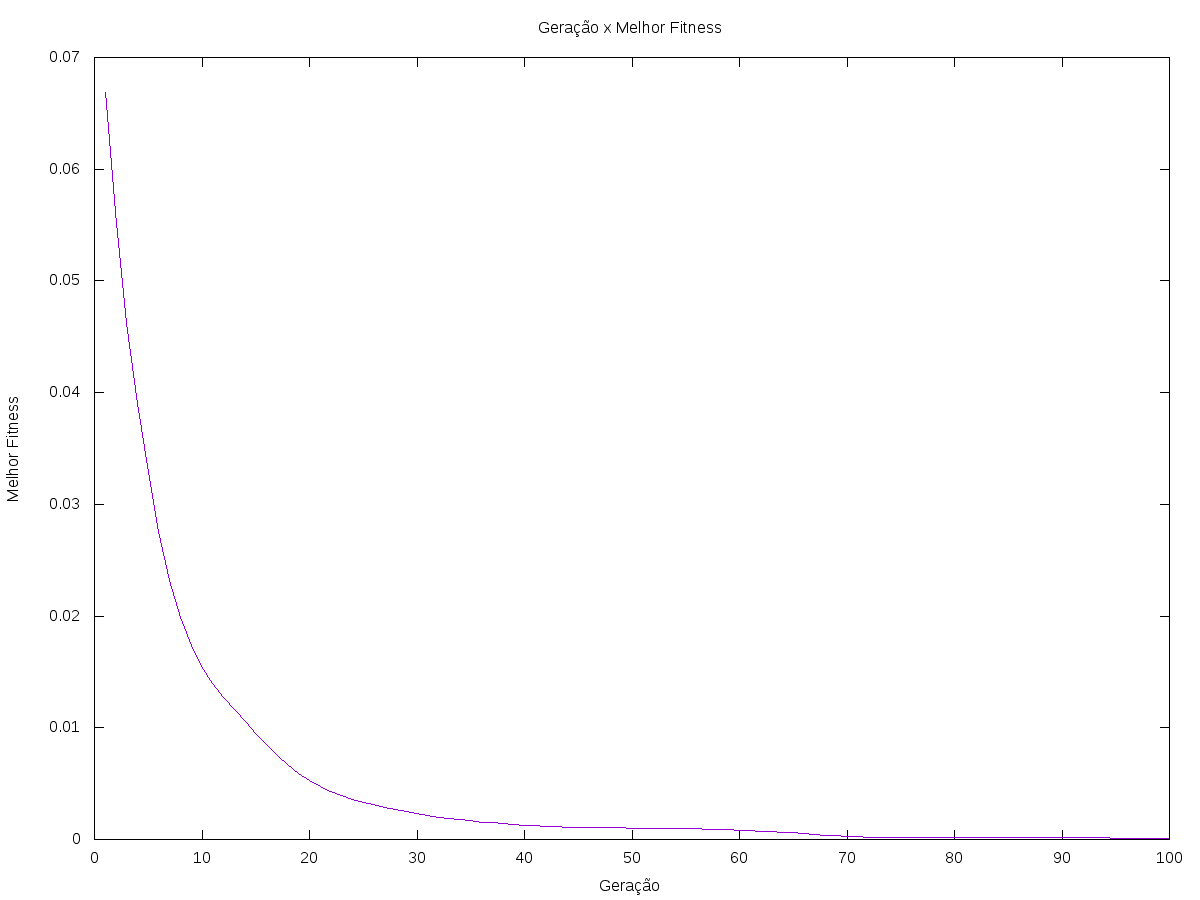
\includegraphics[width=1\textwidth]{exp1k10.png}
  \caption{Experimento 1: Geração x Melhor Fitness para base keijzer-10.}
  \label{fig:exp1k10}
\end{figure}

\begin{figure}[ht]
  \centering
  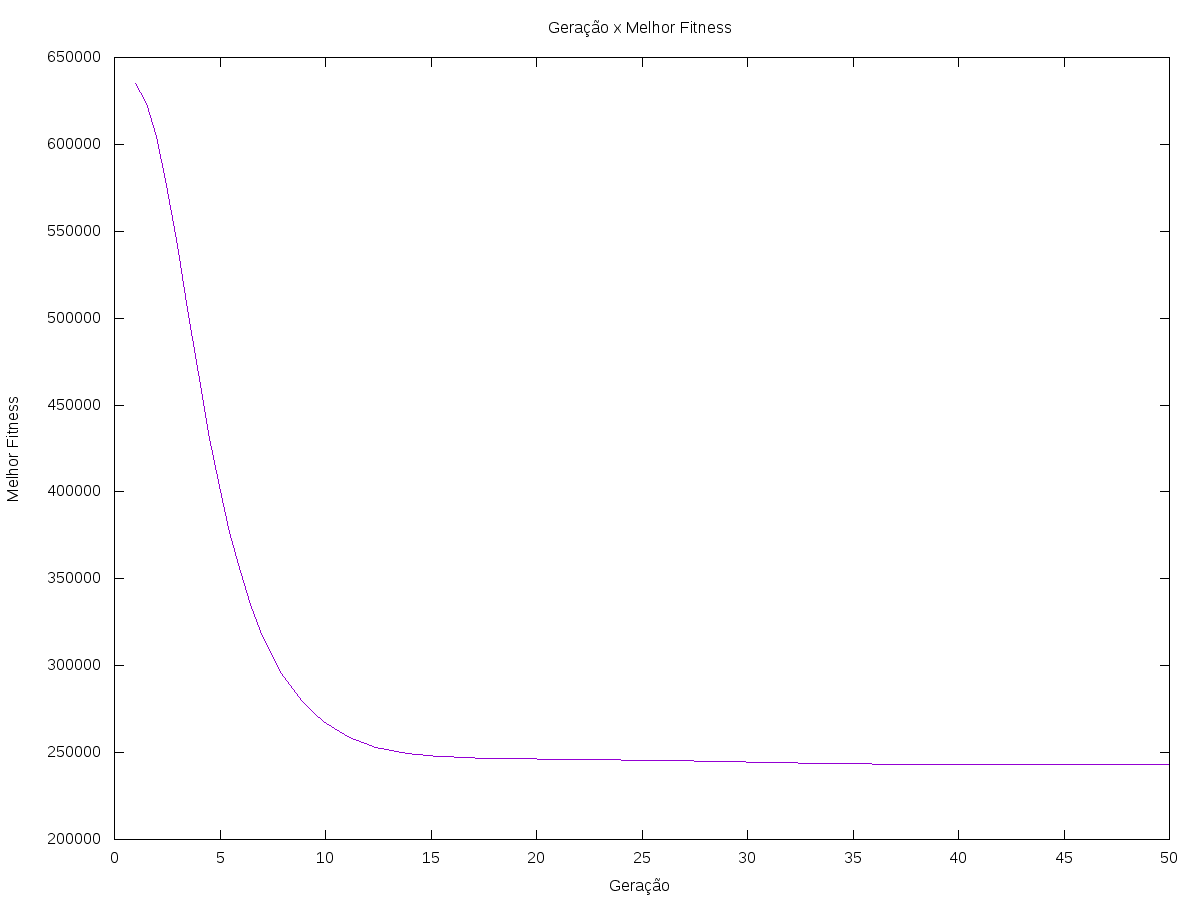
\includegraphics[width=1\textwidth]{exp1h.png}
  \caption{Experimento 1: Geração x Melhor Fitness para base house.}
  \label{fig:exp1h}
\end{figure}
  
Podemos ver que, em um primeiro momento a melhor fitness cai de forma bem acentuada,
em seguida convergindo a um valor específico para cada uma das bases.

\subsection{Experimento 2: Tamanho de população e número de gerações}

A partir do experimento 2 foi possível constatar que o tamanho da população tem grande impacto
na melhor fitness das primeiras gerações. Isso se deve ao fato de que aumentando o número de
invivíduos estamos aumentando a diversidade e explorando melhor o espaço de busca. Também
podemos observar na Figura \ref{fig:exp2h} que, para todos os valores de tamanho de população,
o programa converge para valores muito próximos, e, além disso, isso ocorre sempre por volta da 
geração 30. Concluímos então que o custo adicional de avaliar mais indivíduos não compensa muito
quando vemos que o ponto de convergência é muito próximo para os valores de tamanho de população
testados.

\begin{figure}[ht]
  \centering
  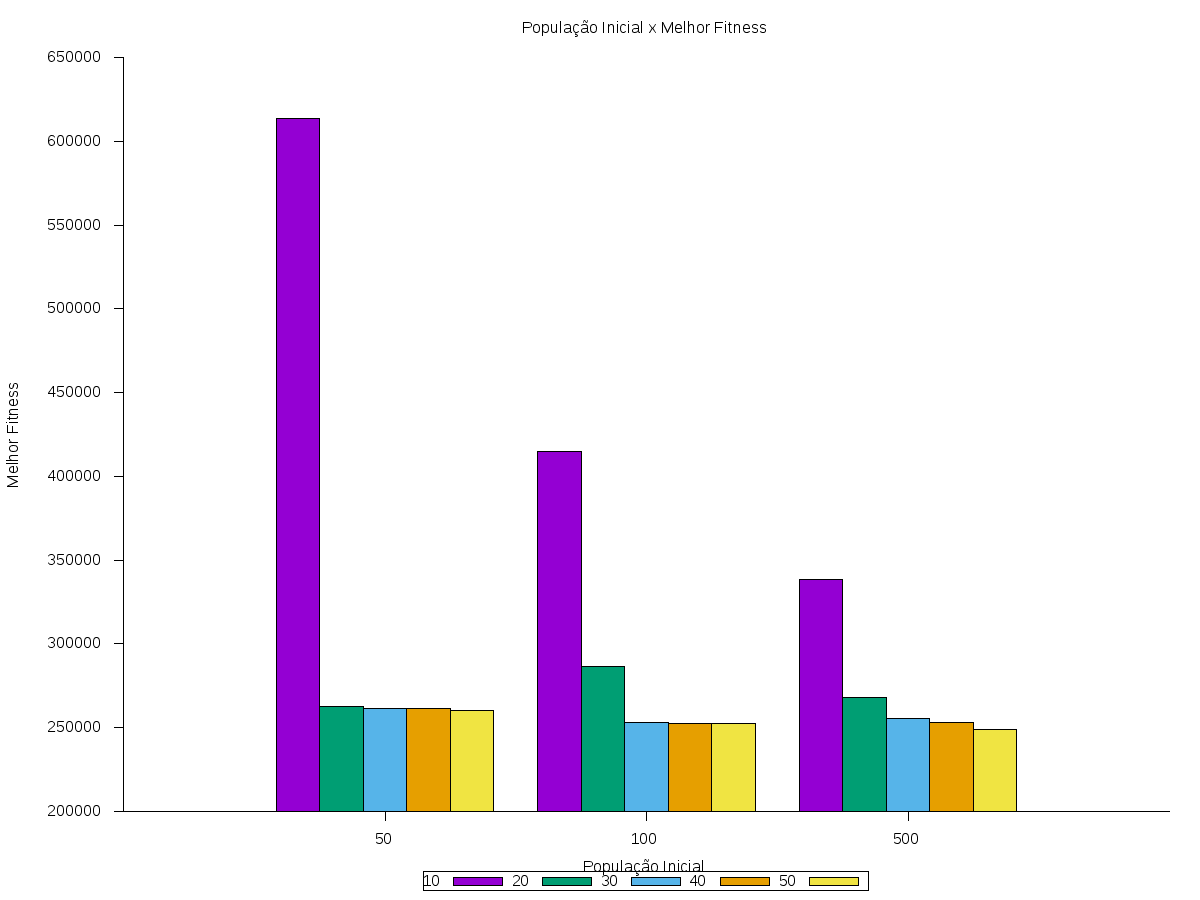
\includegraphics[width=1\textwidth]{exp2h.png}
  \caption{Experimento 2: População inicial x Melhor fitness para cada número de gerações.
  Cada uma das cores representa um número de gerações.}
  \label{fig:exp2h}
\end{figure}

\subsection{Experimento 3: Operadores Genéticos}

\subsection{Experimento 4: Torneio}

\subsection{Experimento 5: Elitismo}

\subsection{Experimento 6: Indivíduos repetidos}

\subsection{Observações}

Os experimentos realizadas possibilitaram observar diversas características importantes, tanto
de Programação Genética em geral, quanto da implementação desse trabalho e das bases de dados
utilizadas.

Vemos que a escolha da probabilidade dos operadores genéticos e tamanho de torneio pode melhorar
a diversidade dos indivíduos, promovendo uma maior exploração do espaço de busca.

Além disso, à medida que a melhor fitness de uma população converge para um determinado valor,
é de se esperar que o número de indivíduos repetidos também tenda a aumentar, dada uma taxa 
de cruzamento alta.

\section{CONCLUSÃO}

O trabalho aqui apresentado foi de grande utilidade para fixar vários conceitos vistos em aula
na disciplina de Computação Natural. Creio que a habilidade de modelar um problema como uma
instância de Programação Genética foi reforçada e poderá ser aplicada com maior facilidade
no futuro.

Pontos chave de aprendizado devem ser ressaltados. Na Programação Genética é importante
definir como representar os indivíduos que representam soluções, e, para isso, é importante
identificar como mapear soluções já conhecidas para soluções genéricas.

Além disso, pode ser constatado que a escolha dos parâmetros do algoritmo afetam significativamente
os resultados obtidos. Sendo o processo de teste algo iterativo, é importante definir a cada
momento a configuração de parâmetros que afeta de maneira mais positiva a saída do programa.

A maior dificuldade encontrada foi lidar com a grande quantidade de testes necessária para
avaliar o projeto. Visto que cada geração pode demorar muito tempo para executar (cada indivíduo
deve ser avaliado e o tamanho da entrada afeta a performance diretamente), foi necessário começar
o processo de testes assim que possível para obter dados e poder analisá-los.

De maneira geral, o aprendizado obtido tem grande apelo, não só para conceitos de Programação Genética,
mas também de Computação Evolucionária em geral.

\section{REFERÊNCIAS}

\bibliographystyle{sbc}
\bibliography{sbc-template}

\end{document}
